% This figure was based on a figure of Izaak Neutelings (September 2020)
\documentclass[border=3pt,tikz]{standalone}
\usepackage{amsmath}
\usepackage{tikz}
\usepackage{physics}
\usepackage[outline]{contour} % glow around text
\usetikzlibrary{calc}
\usetikzlibrary{decorations.markings}
\usetikzlibrary{angles,quotes} % for pic
\usetikzlibrary{arrows.meta} % for arrow size
\usetikzlibrary{bending} % for arrow head angle
\usetikzlibrary{decorations.pathmorphing} % for decorate random steps
\tikzset{>=latex} % for LaTeX arrow head
\usepackage{xcolor}
\contourlength{1.3pt}

\colorlet{xcol}{blue!70!black}
\colorlet{xcol'}{xcol!50!red}
\colorlet{vcol}{green!45!black}
\colorlet{acol}{red!50!blue!80!black!80}
\tikzstyle{rvec}=[->,very thick,xcol,line cap=round]
\tikzstyle{vvec}=[->,very thick,vcol,line cap=round]
\tikzstyle{avec}=[->,very thick,acol,line cap=round]
\colorlet{myred}{red!65!black}
\tikzstyle{force}=[->,myred,very thick,line cap=round]
\tikzstyle{mass}=[line width=0.5,draw=red!50!black,fill=red!50!black!10,rounded corners=1,
                  top color=red!50!black!30,bottom color=red!50!black!10,shading angle=20]
\tikzstyle{disk}=[line width=0.5,orange!30!black,fill=orange!40!black!10,
                  top color=orange!40!black!20,bottom color=orange!40!black!10,shading angle=20]
\tikzstyle{pole}=[line width=0.5,blue!20!black,fill=orange!20!black!10,
                  top color=blue!20!black!20,bottom color=blue!20!black!10,shading angle=20]
\tikzstyle{rope}=[brown!70!black,line width=1,line cap=round] %very thick
\tikzstyle{myarr}=[-{Latex[length=3,width=2,flex'=1]},thin]
\tikzstyle{mydashed}=[dash pattern=on 2pt off 1pt]
\def\rope#1{ \draw[rope,black,line width=1.4] #1; \draw[rope,line width=1.1] #1; }
\def\tick#1#2{\draw[thick] (#1) ++ (#2:0.1) --++ (#2-180:0.2)}
\newcommand\rightAngle[4]{
  \pgfmathanglebetweenpoints{\pgfpointanchor{#2}{center}}{\pgfpointanchor{#3}{center}}
  \coordinate (tmpRA) at ($(#2)+(\pgfmathresult+45:#4)$);
  %\draw[white,line width=0.6] ($(#2)!(tmpRA)!(#1)$) -- (tmpRA) -- ($(#2)!(tmpRA)!(#3)$);
  \draw[black] ($(#2)!(tmpRA)!(#1)$) -- (tmpRA) -- ($(#2)!(tmpRA)!(#3)$);
}


\begin{document}

% SECOND FIGURE: 3D Cartesian axes + omega, v_r, and cross product to show what the coriolis force looks like for someone at the center of the coordinate system positioned on the earth's surface
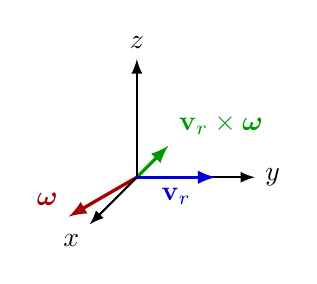
\begin{tikzpicture}
  [
    x={(-0.4cm,-0.4cm)},   % x-axis: out of screen (down-left)
    y={( 1.0cm, 0.0cm)},   % y-axis: right
    z={( 0.0cm, 1.0cm)}    % z-axis: up
  ]

 
  % cross product v_r × omega = (sin30, 0, 0)
  \draw[->,very thick,green!60!black,line cap=round]
    (0,0,0) --
    ({-2*sin(30)},0,0)
    node[pos=1,above right] {$\vb{v}_r \times \vb*{\omega}$};
  % omega vector: (0, -cos30, sin30)
  \draw[force] (0,0,0) --
    (0, {-cos(30)}, {-sin(30)})
    node[pos=1,above left] {$\vb*{\omega}$};


     % axes
  \draw[->,thick] (0,0,0) -- (1.5,0,0) node[below left] {$x$};
  \draw[->,thick] (0,0,0) -- (0,1.5,0) node[right] {$y$};
  \draw[->,thick] (0,0,0) -- (0,0,1.5) node[above] {$z$};

  % v_r vector: (0,1,0)
  \draw[->,very thick,blue!85!black,line cap=round]
    (0,0,0) -- (0,1,0)
    node[pos=0.5,below] {$\vb{v}_r$};

    

  

\end{tikzpicture}



\end{document}